\documentclass[tikz,border=2pt]{standalone}
\usepackage{amsmath,amssymb}
\usepackage{tikz}
\usetikzlibrary{arrows.meta,matrix}

\begin{document}
% A 3x3 Jordan block: lambda on the diagonal, 1s just above it; on the chain basis it acts
% as "scale by lambda and shift one step down the chain".
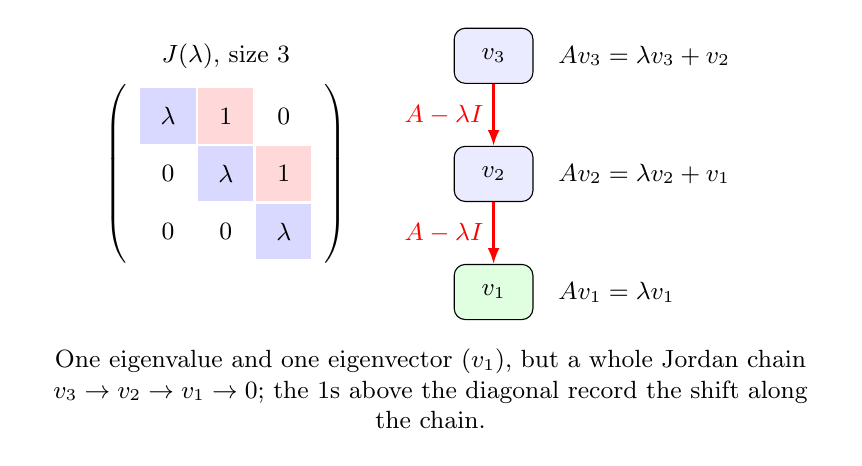
\begin{tikzpicture}[every node/.style={font=\small}, >={Latex[length=2mm]}]
	\matrix (J) [matrix of math nodes, nodes={minimum size=7mm, anchor=center}, left delimiter=(, right delimiter=), column sep=1pt, row sep=1pt] at (0,0) {
		|[fill=blue!15]| \lambda & |[fill=red!15]| 1 & 0 \\
		0 & |[fill=blue!15]| \lambda & |[fill=red!15]| 1 \\
		0 & 0 & |[fill=blue!15]| \lambda \\
	};
	\node[anchor=south] at (J.north) {$J(\lambda)$, size $3$};
	\begin{scope}[xshift=3.4cm]
		\node[draw, rounded corners=4pt, fill=blue!8, minimum width=1.0cm, minimum height=0.7cm] (v3) at (0,1.5) {$v_3$};
		\node[draw, rounded corners=4pt, fill=blue!8, minimum width=1.0cm, minimum height=0.7cm] (v2) at (0,0) {$v_2$};
		\node[draw, rounded corners=4pt, fill=green!12, minimum width=1.0cm, minimum height=0.7cm] (v1) at (0,-1.5) {$v_1$};
		\draw[->, thick, red] (v3) -- (v2) node[midway, left] {$A-\lambda I$};
		\draw[->, thick, red] (v2) -- (v1) node[midway, left] {$A-\lambda I$};
		\node[anchor=west] at (0.7,1.5) {$Av_3=\lambda v_3+v_2$};
		\node[anchor=west] at (0.7,0) {$Av_2=\lambda v_2+v_1$};
		\node[anchor=west] at (0.7,-1.5) {$Av_1=\lambda v_1$};
	\end{scope}
	\node[anchor=north, align=flush center, text width=10cm] at (2.6,-2.1) {One eigenvalue and one eigenvector ($v_1$), but a whole Jordan chain $v_3\to v_2\to v_1\to0$; the $1$s above the diagonal record the shift along the chain.};
\end{tikzpicture}
\end{document}
